%%%%%%%%%%%%%%%%%%%%%%%%%%%%%%%%%%%%%%%%%%%%%%%%%%%%%%%%%%%%%%%%%%%%%%%%%%%%%%%%%%%%%%%%%
%%                                                                                     %%
%%                This file is part of the CAPH Compiler distribution                  %%
%%                            http:%/caph.univ-bpclermont.fr                           %%
%%                                                                                     %%
%%                                  Jocelyn SEROT                                      %%
%%                         Jocelyn.Serot@univ-bpclermont.fr                            %%
%%                                                                                     %%
%%         Copyright 2011-2018 Jocelyn SEROT.  All rights reserved.                    %%
%%  This file is distributed under the terms of the GNU Library General Public License %%
%%      with the special exception on linking described in file ..%LICENSE.            %%
%%                                                                                     %%
%%%%%%%%%%%%%%%%%%%%%%%%%%%%%%%%%%%%%%%%%%%%%%%%%%%%%%%%%%%%%%%%%%%%%%%%%%%%%%%%%%%%%%%%%

\chapter{Compilation options}
\label{cha:ide-options}

The caph compiler comes with a fairly large number of options (see Sec. 12 of the language reference
manual). Most of these options can be set and inspected by invoking \textsf{Compilater options} item
of the \textsf{Configuration} menu. Options are organized by grouped by tabs, as illustrated in
Fig.~\ref{fig:options-sysc}, in which the tab related to SystemC has been selected.

\begin{figure}[h]
  \centering
  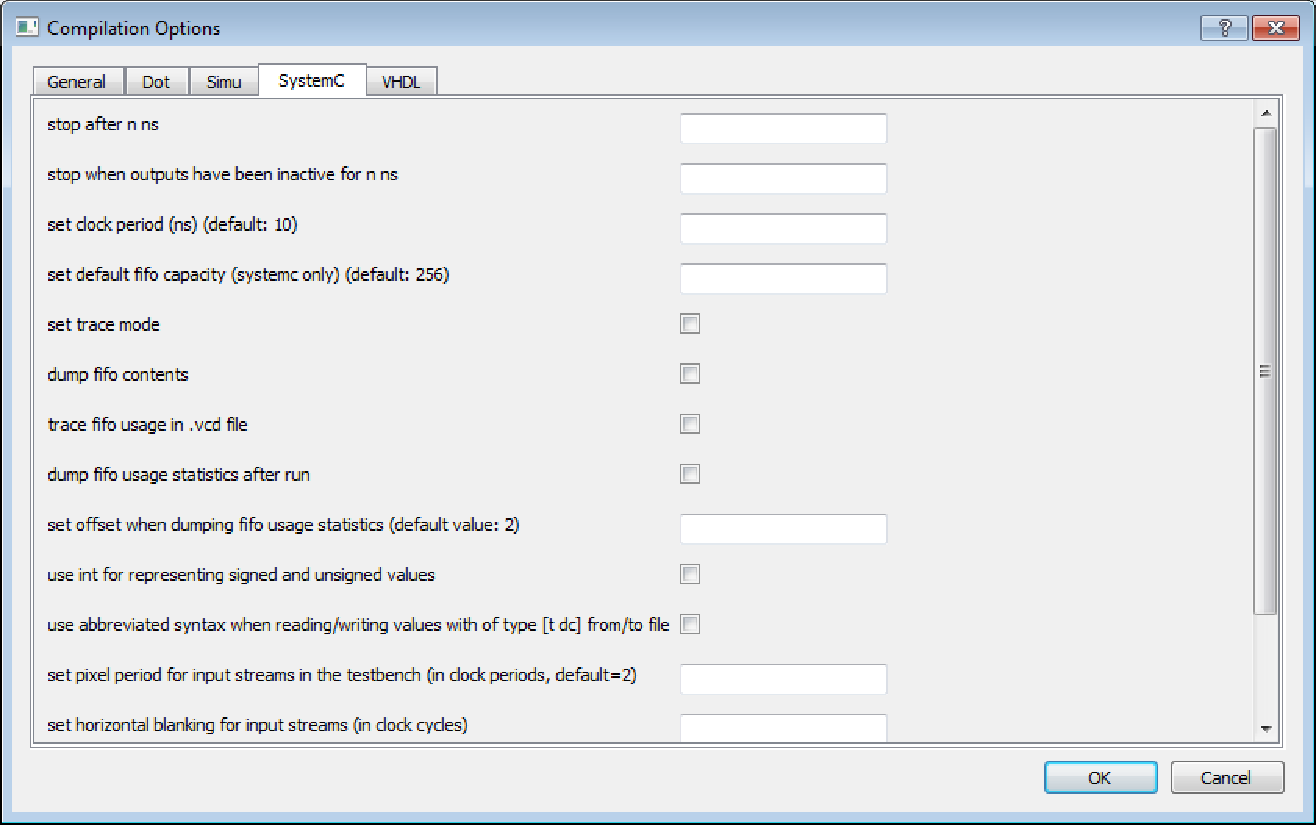
\includegraphics[width=0.75\textwidth]{figs/ide/options-sysc}
  \caption{The options setting dialog}
  \label{fig:options-sysc}
\end{figure}

\medskip An important point is that, when working in project mode, each modification to compilation
options is recorded and saved in a dedicated file in the project directory. This file, when present,
is automatically read when a project is opened. This way, compilation options are remembered between
sessions.

%%% Local Variables: 
%%% mode: latex
%%% TeX-master: "caph-primer"
%%% End: 
